% Name: Radar chart
% Description: Two products scored from 0 to 5 on six criteria, drawn as overlapping polygons on a spider web of rings and spokes.
% Tags: radar chart, spider chart, comparison, scores

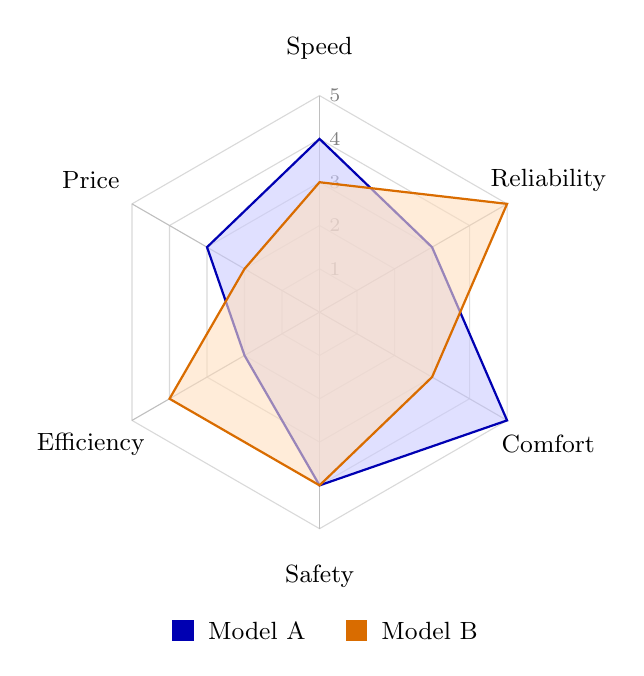
\begin{tikzpicture}[font=\small, scale=0.55]
  % Spoke i points at 90 - 60i degrees; one unit of score is one unit of radius.
  \foreach \r in {1,...,5}
    \draw[gray!30] (90:\r) \foreach \i in {1,...,5} { -- (90-60*\i:\r) } -- cycle;
  \foreach \name [count=\i from 0] in {Speed, Reliability, Comfort, Safety, Efficiency, Price} {
    \draw[gray!50] (0,0) -- (90-60*\i:5);
    \node at (90-60*\i:6.1) {\name};
  }
  \foreach \r in {1,...,5} \node[gray, font=\scriptsize, right] at (90:\r) {\r};
  \filldraw[blue!70!black, fill=blue!20, fill opacity=0.6, thick]
    (90:4) \foreach \v [count=\i] in {3,5,4,2,3} { -- (90-60*\i:\v) } -- cycle;
  \filldraw[orange!85!black, fill=orange!25, fill opacity=0.6, thick]
    (90:3) \foreach \v [count=\i] in {5,3,4,4,2} { -- (90-60*\i:\v) } -- cycle;
  \fill[blue!70!black] (-3.4,-7.6) rectangle ++(0.5,0.5);
  \node[right] at (-2.8,-7.35) {Model A};
  \fill[orange!85!black] (0.6,-7.6) rectangle ++(0.5,0.5);
  \node[right] at (1.2,-7.35) {Model B};
\end{tikzpicture}
